\documentclass[11pt, spanish, a4paper, twopage]{article}

% Versión 1.er cuat 2021 Víctor Bettachini < vbettachini@unlam.edu.ar >

\usepackage[T1]{fontenc}
\usepackage[utf8]{inputenc}

\usepackage[spanish, es-tabla]{babel}
\def\spanishoptions{argentina} % Was macht dass?
% \usepackage{babelbib}
% \selectbiblanguage{spanish}
% \addto\shorthandsspanish{\spanishdeactivate{~<>}}

\usepackage{graphicx}
\graphicspath{{./figuras/}{../LaTeX/}}
% \usepackage{float}

\usepackage[arrowdel]{physics}
\newcommand{\pvec}[1]{\vec{#1}\mkern2mu\vphantom{#1}}
% \usepackage{units}
\usepackage[separate-uncertainty= true, multi-part-units= single, range-units= single, range-phrase= {~a~}, locale= FR]{siunitx}
\usepackage{isotope} % $\isotope[A][Z]{X}\to\isotope[A-4][Z-2]{Y}+\isotope[4][2]{\alpha}

\usepackage{tasks}
\usepackage[inline]{enumitem}
% \usepackage{enumerate}

\usepackage{hyperref}

% \usepackage{amsmath}
% \usepackage{amstext}
% \usepackage{amssymb}

\usepackage{tikz}
\usepackage{tikz-dimline}
\usetikzlibrary{calc}
% \usetikzlibrary{math}
\usetikzlibrary{arrows.meta}
\usetikzlibrary{snakes}
\usetikzlibrary{decorations}
\usetikzlibrary{decorations.pathmorphing}
\usetikzlibrary{patterns}

\usepackage[hmargin=1cm,vmargin=3cm, top= 0.75cm,nohead]{geometry}

\usepackage{lastpage}
\usepackage{fancyhdr}
\pagestyle{fancyplain}
\fancyhf{}
\setlength\headheight{28.7pt} 
\fancyhead[LE, LO]{\textbf{Mecánica General} }
\fancyhead[RE, RO]{\href{https://ingenieria.unlam.edu.ar/}{$\vcenter{\hbox{
\includegraphics[height=1cm]{ambos.pdf}}}$}}
\fancyfoot{\href{https://creativecommons.org/licenses/by-nc-sa/4.0/deed.es_ES}{$\vcenter{\hbox{
\includegraphics[height=0.4cm]{by-nc-sa_80x15.pdf}}}$} \href{https://ingenieria.unlam.edu.ar/}{DIIT - UNLaM}}
\fancyfoot[C]{ {\tiny Actualizado al \today} }
\fancyfoot[RO, LE]{Pág. \thepage/\pageref{LastPage}}
\renewcommand{\headrulewidth}{0pt}
\renewcommand{\footrulewidth}{0pt}


\begin{document}
\begin{center}
  % \textsc{\large Mecánica general}\\
  \textsc{\large Cinemática y dinámica Newtoniana de la partícula puntual}
\end{center}

%De poder resolver estos problemas en forma autónoma puede asumir que adquirió los conocimientos mínimos sobre los temas abordados.
%No dude en consultar a docentes y compañeros si no puede terminarlos.
% Los problemas marcados con * son opcionales.
\begin{enumerate}


\section*{Ecuaciones de la dinámica - 2"a ley de Newton}


\item
\textbf{Las fuerzas conservativas, las dependientes de un potencial | Péndulo}\\
\begin{minipage}[t][1.8cm]{0.73\textwidth}
%\textbf{Péndulo} [Marion () ex. 7.2] \\
Obtenga la ecuación diferencial que describe la dinámica de una pesa que ``pendulea'' en el extremo de una cuerda.
\end{minipage}
\begin{minipage}[c][3.2cm][t]{0.2\textwidth}
%	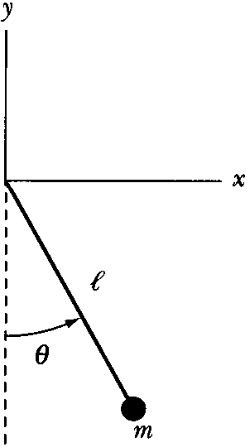
\includegraphics[width=\textwidth]{marion_fig7_1}
%	\includegraphics[width=\textwidth]{\detokenize{pénduloHorizontal}}
	\begin{tikzpicture}[scale= 1.0]
	\draw [arrows=-latex] (-1,2) -> (-1,1) node [above=15, right=2] {\(\vec{g}\)}; % g vertical
		\draw [ultra thick] (-1.5,3) -- (2,3);
		\fill [pattern = north east lines] (-1.5,3) rectangle (2,3.2); % techo
		\draw [dashed] (0,3) -- (0,-.25);	% vertical
		\draw [thick] (0,3) -- +(-60:3) node[midway,above,right=2] {\(\ell\)};	% inclinada +:relativa, -60 grados, longitud 3
		\shade [ball color=black!80] ($(0,3)+(-60:3)$) circle(0.25) node [] {\color{white} $m$};
    \draw [arrows=-latex] (0,.4) -> (1.25,.4) node [midway, above] {\( \psi \)}; % desplazamiento horizontal
		\draw [arrows=-latex] (0,0) arc [start angle=-90, end angle=-65, radius=3] node [below=12, left=8] {\( \varphi \)};
	\end{tikzpicture}
\end{minipage}
\begin{enumerate}
	\item Asumiendo que el péndulo oscila dentro del plano \(\hat{x}, \hat{y}\).
		¿En que sistema de coordenadas resolverá el problema? 
		¿Cuál coordenada es relevante para describir la dinámica? 
	\item Enumere las aproximaciones del modelo de péndulo que resolverá que lo diferencian de uno que puede armar en el laboratorio.
	\item Calcule la energía potencial de la pesa en el campo gravitatorio.
	¿Para qué sirve eso?
	Las fuerzas que surgen de un campo son fácilmente calculables usando que \(\vec{F} = - \vec{\nabla} V\), es decir, \emph{la fuerza es igual al negativo del gradiente del potencial}.
	\item Escriba la 2.a ley de Newton y proyecte en la dirección de la coordenada relevante.
	\item Resuelva la ecuación de la dinámica y obtenga la frecuencia de oscilación.
\end{enumerate}
%\vspace{-2.5cm}


%\subsection*{Fuerza como gradiente de un potencial}
%% Vizcaino carpeta
%\item Una partícula esta sometida a una fuerza \(\vec{F}(x)= \left( -k x + \frac{a}{x^3}\right) \hat{x}\)
%\begin{enumerate}
%    \item Hallar el potencial \(U(x)\) y graficarlo.
%    \item Discutir los tipos de movimientos posibles.
%    \item Determinar las posiciones de equilibrio estable y encuentre la solución general de la dinámica de la partícula, \(\vec{r}(t)\).
%    \item Interpretar el movimiento en el límite \(E^2 \gg k a\). ¿Cuanto vale el periodo de las oscilaciones?
%    \item Ídem. anterior en el límite \(E^2 \rightarrow k a\) con \(E^2 > k a\).
%\end{enumerate}



%\item
%\begin{minipage}[t][6.5cm]{0.6\textwidth}
%\textbf{Marion e.g. 2.10} Particula cargada en \(\va{B}\) constante
%
%La fuerza de Lorentz es la ejercida a una particular de carga eléctrica \(q\) por un campo eléctrico \(\vec{E}\) y magnético \(\vec{B}\):
%\[
%	\vec{F}= q \left( \vec{E}+ \vec{v} \cross \vec{B} \right).
%\]
%La figura muestra esquemáticamente una trayectoria y las condiciones \(\va{v}_0, \va{B}=\mathrm{cte}.\) que le dieron lugar.
%Halle las ecuaciones de tal dinámica.
%\end{minipage}
%\begin{minipage}[c][0cm][t]{0.35\textwidth}
%	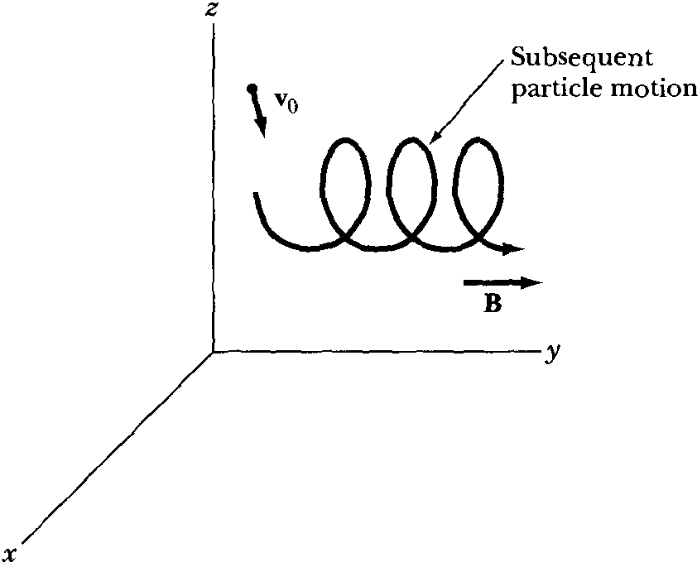
\includegraphics[width=\textwidth]{marionFig2_12.png}
%\end{minipage}
%



\section*{Condiciones de vínculo}
\item
\begin{minipage}[t][5cm]{0.4\textwidth}
\textbf{Máquina de Atwood} [Marion (e) ex. 2.9]\\
Esta máquina consiste de una polea sin fricción de la que suspenden dos masas al final de cada extremo de un hilo.
Encuentre la aceleración de las masas y la tensión de las cuerda:
  \begin{enumerate}
	\item cuando el centro de la polea está en reposo,
	\item y cuando la polea desciende en un ascensor con aceleración constante \(a\).
  \end{enumerate}
\end{minipage}
\begin{minipage}[c][1cm][t]{0.55\textwidth}
	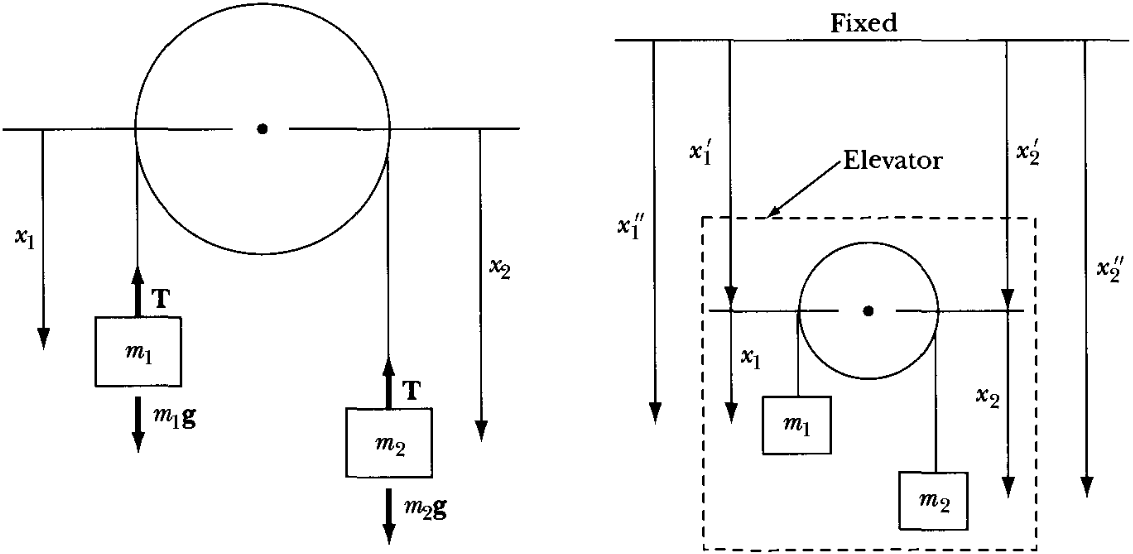
\includegraphics[width=\textwidth]{marionFig2_11.png}
\end{minipage}
%\vspace{1cm}

%\item
%\begin{minipage}[t][3.5cm]{0.75\textwidth}
%Máquina de Atwood % \textbf{Vizcaino 1.1} 
%
%El sistema de la figura esta inicialmente en reposo, las poleas tienen masa despreciable y los hilos son inextensibles.
%  \begin{enumerate}
%   \item Halle la aceleración de cada cuerpo y las tensiones en los hilos en función de \(m_1\), \(m_2\), \(m_3\), y \(g\).
%   \item Resuelva a) para el caso \(m_1= \SI{4}{\kilo\gram}\), \(m_2= \SI{2}{\kilo\gram}\) y \(m_3= \SI{1}{\kilo\gram}\).
%  \end{enumerate}
%\end{minipage}
%\begin{minipage}[c][0em][t]{0.15\textwidth}
%        \includegraphics[width=\textwidth]{atwood-prob}
%\end{minipage}


\section*{Conservación del momento lineal}

% FCEyN 0.1
\item 
\begin{minipage}[t][1.8cm]{0.65\textwidth}
Una barra rígida de longitud \(\ell\) conecta dos esferas de masa \(m_1\) y \(m_2\).
Sobre una superficie se apoya la de \(m_1\) pero se sostiene la barra formando un ángulo \(\theta\) con la horizontal.
La superficie no presenta rozamiento a las esferas.
Considere las esferas puntuales y despreciable la masa de la barra.
\end{minipage}
\begin{minipage}[c][0.3cm][t]{0.3\textwidth}
	\begin{tikzpicture}[scale= 1]
		\def \radioEsfera{0.25};
		\def \barraAngulo{15};
		\coordinate (m1) at (-2,0);
		% \coordinate (m2) at (2,1);
		\coordinate (m2) at ($(m1) + (\barraAngulo:4)$);
		\draw [dashed] (m1) -- ($(m1) + (4,0) $); % referencia theta
		\draw [-latex] ($(m1) + (3,0) $) arc(0 : \barraAngulo : 3) node [midway, right] {$\theta$};
		\draw [very thick](m1)--(m2) node [midway, above] {$\ell$}; % barra
		\shade [ball color=black!80] (m1) circle(\radioEsfera) node [] {\color{white} $m_1$};
		\shade [ball color=black!80] (m2) circle(\radioEsfera) node [] {\color{white} $m_2$};
		\def \sueloLargo{5.25};
		\def \sueloProfundidad{0.15};
		\coordinate (sueloArribaIzquierda) at (-2.75, -\radioEsfera);
		\draw [ultra thick] (sueloArribaIzquierda) -- ($(sueloArribaIzquierda) + (\sueloLargo,0) $); % suelo
		\fill [pattern = north east lines] (sueloArribaIzquierda) rectangle ($ (sueloArribaIzquierda) + (\sueloLargo, -\sueloProfundidad) $); % suelo
	\end{tikzpicture}
\end{minipage}

Pregunta coneceptual:
No hay rozamiento. ¿Qué sucede entonces con el momento en la dirección horizontal?
¿Qué consecuencia tiene esto en la coordenada horizontal del centro de masa?

\textbf{Determine}:
Donde golpea \(m_2\) a la superficie tras dejar en libertad a la barra.



%\subsection*{Momento angular}
%% FCEN 0.6
%% Problema horripilante, pues se resuelve como uno de fuerza central, hay que encontrar uno mas simple sobre conservación de momento angular.
%\item Dos partículas de masas \(m_a\) y \(m_b\) están sobre una mesa horizontal sin fricción.
%Se encuentran unidas por una cuerda tensa que pasa por un anillo pequeño fijo a la mesa, que tampoco presenta fricción a la cuerda. Inicialmente las partículas están quietas a distancias \(R_a\) y \(R_b\) del anillo y en \(t = 0\) se le da un impulso a la masa \(m_b\), perpendicular a la cuerda, de modo que esta adquiere una velocidad \(v_0\).
%\begin{enumerate}
%    \item ¿Qué magnitudes se conservan?
%    \item Dar la velocidad de las partículas en función de su distancia al anillo.
%    \item Hallar la tensión de la cuerda en función de la distancia de una masa al anillo.
%\end{enumerate}



\section*{Coordenadas polares}

\item
\begin{minipage}[t][2cm]{0.6\textwidth}
\textbf{Masa resbalando sobre semi-esfera}\\ 
La partícula de masa \(m\), considerada puntual, desliza sobre una semi-esfera de radio \(R\) sin fricción.
\end{minipage}
\begin{minipage}[c][1cm][t]{0.3\textwidth}
	% \includegraphics[width=\textwidth]{marion7_10}
	\begin{tikzpicture}[scale= 1]
		\draw [ultra thick] (-3,0) -- (3,0);
		% \draw [ultra thick] (-3,0) -- (3,0);
		\fill [pattern = north east lines] (-3,0) rectangle (3,-0.2); % piso
		\draw [ultra thick] (-2,0) .. controls (-2,2*0.555) and (-2*0.555,2) .. (0,2) .. controls (2*0.555,2) and (2,2*0.555) .. (2,0); % semi esfera
		% \filldraw (0,2.2) circle (0.2); % masa superior
		% \fill (2*0.5+.12,1.732+.18) circle [radius=0.25] node [midway, text=white] { \( m \) };
		% \filldraw (2*0.5+.12,1.732+.18) circle (0.2) node [above, right=5] {\(m\)}; % masa a la derecha
		\shade [ball color=black!80] (2*0.5+.12,1.732+.18) circle(0.2) node [] {\color{white} $m$};
		% \draw (2,2) circle [radius=0.3, color=white, fill=black] node {$T_1$};
		\draw [dashed] (0,0) -- (0,2); % linea vertical
		\draw [-LaTeX] (0,0) -- (1,1.732) node [midway, anchor=west] {\(R\)}; % linea hacia la derecha
		\draw [-stealth] (0,1) arc (90:60:1) node [above left] {\(\theta\)}; % arco c/ flecha comenzando en (0,1), de 90 a 60 grados, 1...
		% \node [circle,draw,label=60:$60^\circ$,label=below:$-90^\circ$] {\(m\)}; 
		% \node at (-2*0.5+.15,1.732+.15) [circle,draw,fill=black] {\(m\)}; 
		\draw [-stealth, thick] (-2.5,2) -> (-2.5,1) node [above=15, right=2] {\(\vec{g}\)}; % g vertical
	\end{tikzpicture}
\end{minipage}
\begin{enumerate}
	\item Calcular el ángulo \(\theta\) para el cual se separa de semi-esfera si inicialmente es apartada en un ángulo muy pequeño de \(\theta= 0\) y su velocidad inicial es nula.
	\item Si la partícula estuviera engarzada sin fricción en un riel semi-circular de radio \(R\), hallar la velocidad con que llega al suelo.
¿Qué aceleración tangencial tiene en ese momento?
\end{enumerate}




\section*{Conservación del momento angular}

\item \textbf{Ratón en ventilador de techo} [Marion (e) ex. 2.11]\\
El conjunto de aspas de un ventilador de techo tiene momento de inercia \(I\) y radio \(R\).
Mientras estas giran a velocidad constante en el borde externo de una de ellas asoma un ratón de masa \(m\).
En un dado momento este salta.
A causa de esto, ¿cuanto cambiará la velocidad angular del ventilador respecto a la que tenía antes?




% \section*{Sistema no inercial - sistema en rotación}
% % FCEyN 0.4
% \item Un disco homogéneo de masa \(M\) y radio \(R\) está girando con velocidad angular \(\omega \).
% % Una mosca de masa \(m\) que inicialmente se encuentra en el centro del disco camina radialmente hacia afuera con velocidad relativa constante.
% \begin{enumerate}
% \item Si el disco es obligado a girar con velocidad relativa constante por un motor, ¿qué torque debe hacer éste para compensar el movimiento de la mosca?
% ¿Cúal es la fuerza de Coriolis que siente la mosca?
% \item Si el disco gira libremente, ¿cúal será la velocidad angular del disco cuando la mosca está a una distancia \(d\) del centro?
% \end{enumerate}


%\item \setlength{\parskip}{0cm} % OLVIDÉ DE QUE TRATA ESTE PROBLEMA
%  \begin{enumerate}
%  \item Considere un resorte de constante elástica \(k\), sin masa y sin rozamiento, fijo de un extremo y obligado a moverse según una fuerza \(F_1\) de tal modo que \(x = x_0 \cos(\omega t)\)
%¿Cuánto debe valer \(F_1\)? (\(x\) se mide desde la posición de equilibrio).
%  \item Un cuerpo de masa \(m\) es movido por una fuerza \(F_2\) de tal modo que \(x = x_0 \cos(\omega t)\), ¿Cuánto vale \(F_2\)?
%  \item La masa \(m\) de b) se fija al extremo libre del resorte de a), y el sistema es obligado a moverse por una fuerza \(F_3\) de tal modo que la masa ejecuta un movimiento \(x = x_0 \cos(\omega t)\) ¿Cuánto vale \(F_3\)?
%  \item Si \(\omega = \omega_0 = \sqrt{\frac{k}{m}}\), ¿Cuánto vale \(F_3\)?
%  \item Estudie los límites \(\omega \gg \omega_0\) y \(\omega \ll \omega_0\), determine \(F_3\) y diga si el sistema se comporta como en a) o como en b).
%  \end{enumerate}



%\subsection*{Fuerzas no provenientes de un potencial}
%
%\item
%\begin{minipage}[t][6cm]{0.5\textwidth}
%% \textbf{MIT2_003SCF11_pset3_e02}
%El cabrestante, que se muestra en la figura, entrega una fuerza de tirado horizontal, $T(t)$, a su cable en $D$.
%La fuerza varía con el tiempo, como se muestra en el gráfico.
%La pesa de masa \(M\) de \SI{80}{\kilo\gram} en \(t=0\) estaba en reposo.
%Para simplificar el problema se asume que las poleas y cables tienen masa despreciable.
%\begin{enumerate}
%	\item Pregunta conceptual:
%	¿Espera que la velocidad de la masa sea constante mientras la fuerza es constante durante el intervalo de 0 a 12 segundos?\\
%	\begin{enumerate*}[label=\alph*),itemjoin={,\quad}]
%		\item Sí
%		\item No
%		\item No sé qué principio aplicar.
%	\end{enumerate*}
%	\item Determine la velocidad de la pesa en $t=\SI{24}{\second}$.
%\end{enumerate}
%\end{minipage}
%\begin{minipage}[c][0cm][t]{0.45\textwidth}
%	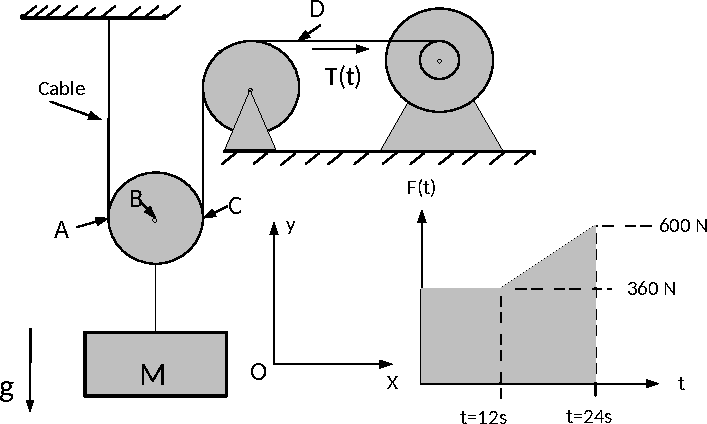
\includegraphics[width=\textwidth]{MIT2_003SCF11_pset3_e02}
%\end{minipage}




\end{enumerate}
\end{document}
